%%%%%%%%%%%%%%%%%%%%%%%%%%%%%%%%%%%%%%%%%%%%%%%%%%%%%%%%%%%%%%%%%%%%%%%%%%%%%%%%%%
\begin{frame}[fragile]\frametitle{}
\begin{center}
{\Large Overview of Large Language Models}
\end{center}
\end{frame}

%%%%%%%%%%%%%%%%%%%%%%%%%%%%%%%%%%%%%%%%%%%%%%%%%%%%%%%%%%%
\begin{frame}[fragile]\frametitle{What is a Language Models?}

\begin{itemize}
\item While typing SMS, have you seen it suggests next word?
\item While typing email, have you seen next few words are suggested?
\item How does it suggest? (suggestions are not random, right?)
\item In the past, for ``Lets go for a \ldots', if you have typed 'coffee' 15 times, 'movie' say 4 times, then it learns that. Machine/Statistical Learning.
\item Next time, when you type ``Lets go for a '', what will be suggested? why?
\item This is called Language Model. Predicting the next word. When done continuously, one after other, it spits sentence, called Generative Model.
\end{itemize}	

\begin{center}
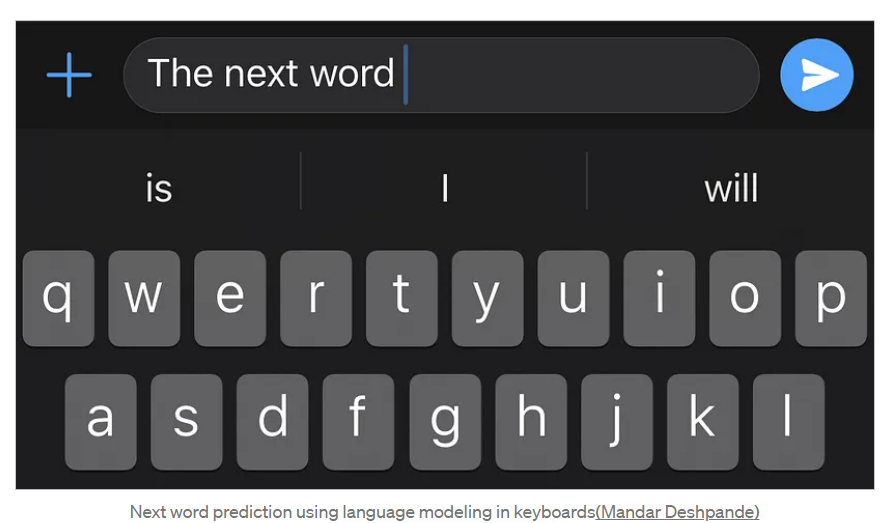
\includegraphics[width=0.6\linewidth,keepaspectratio]{chatgpt34}
\end{center}		

\end{frame}

%%%%%%%%%%%%%%%%%%%%%%%%%%%%%%%%%%%%%%%%%%%%%%%%%%%%%%%%%%%
\begin{frame}[fragile]\frametitle{Overview}


\begin{itemize}
\item Large Language Models (LLMs) are deep neural networks (e.g., GPT-3, BERT) based on the Transformer architecture.
\item LLMs are foundation models trained on large amounts of unsupervised and unstructured data.
\item The Transformer architecture consists of an encoder and decoder, both mostly identical with a few differences.
\item LLMs compute a probability distribution over a vocabulary (list of tokens) given an input prompt.
\item LLMs have limitations like hallucination and issues in chain of thought reasoning, but recent improvements have been made.
\item LLMs are trained for statistical language modeling, which involves predicting the next token based on context.
\end{itemize}

				
{\tiny (Ref: Overview of Large Language Models - Aman AI)}

\end{frame}


%%%%%%%%%%%%%%%%%%%%%%%%%%%%%%%%%%%%%%%%%%%%%%%%%%%%%%%%%%%
\begin{frame}[fragile]\frametitle{Evolution of Language Models}

Language Models can be statistical (frequency based) or Machine/Deep Learning (supervised) based. Simple to complex.

\begin{center}
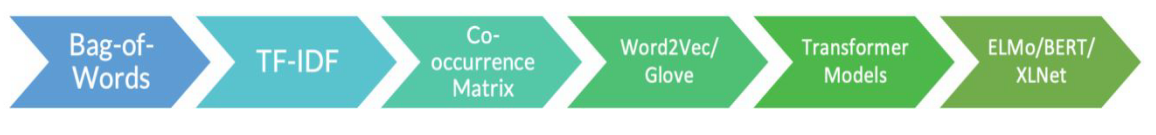
\includegraphics[width=\linewidth,keepaspectratio]{chatgpt30}
\end{center}				
{\tiny (Ref: Analytics Vidhya https://editor.analyticsvidhya.com/uploads/59483evolution\_of\_NLP.png)}

\end{frame}

%%%%%%%%%%%%%%%%%%%%%%%%%%%%%%%%%%%%%%%%%%%%%%%%%%%%%%%%%%%
\begin{frame}[fragile]\frametitle{Large Language Models - Comparison}

\begin{center}
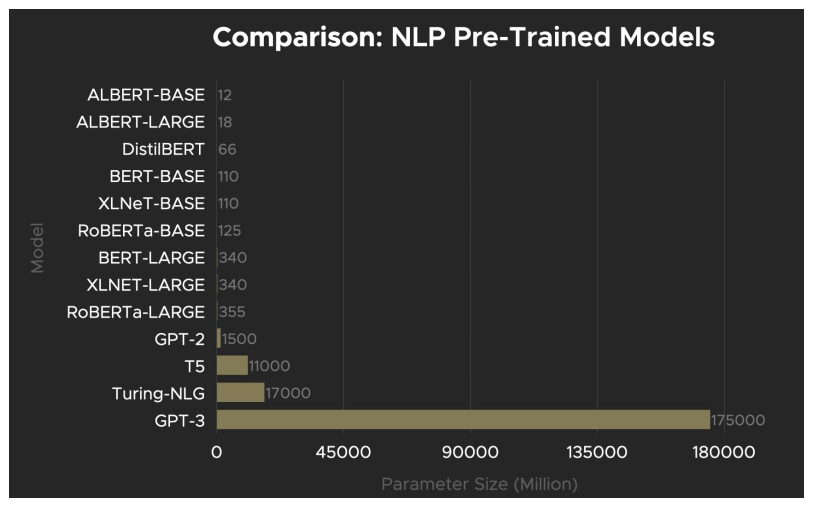
\includegraphics[width=\linewidth,keepaspectratio]{chatgpt31}
\end{center}				
{\tiny (Ref: Deus.ai https://www.deus.ai/post/gpt-3-what-is-all-the-excitement-about)}

\end{frame}

%%%%%%%%%%%%%%%%%%%%%%%%%%%%%%%%%%%%%%%%%%%%%%%%%%%%%%%%%%%
\begin{frame}[fragile]\frametitle{How Do LLMs Work?}


\begin{itemize}
\item LLMs predict the next token based on previous tokens in an autoregressive manner for generation.
\item The prompt is tokenized and converted into non-contextualized embeddings.
\item Layer-by-layer attention and feed-forward computations are performed.
\item Decoder models assign logits to words in the vocabulary or output contextualized embeddings for encoder models.
\item For decoder models, logits are converted into a probability distribution using Softmax.
\item The probability distribution determines the next word in the generated text.
\end{itemize}

				
{\tiny (Ref: Overview of Large Language Models - Aman AI)}

\end{frame}

%%%%%%%%%%%%%%%%%%%%%%%%%%%%%%%%%%%%%%%%%%%%%%%%%%%%%%%%%%%
\begin{frame}[fragile]\frametitle{LLM Training Steps}

At a top-level, here are steps involved in training LLMs:

\begin{itemize}
\item Corpus Preparation: Gather a large corpus of text data from various sources.
Tokenization: Split the text into individual words or subword units (tokens).
Embedding Generation: Generate embeddings using random initialization or pre-trained embeddings like Word2Vec, GloVe, or FastText.
Neural Network Training: Train a neural network model on the input tokens.
\begin{itemize}
\item For encoder models (e.g., BERT), predict the context of a given word through masked language modeling and next sentence prediction tasks.
\item For decoder models (e.g., GPT-N), predict the next token in the sequence based on prior context.
\end{itemize}
\end{itemize}

				
{\tiny (Ref: Overview of Large Language Models - Aman AI)}

\end{frame}

%%%%%%%%%%%%%%%%%%%%%%%%%%%%%%%%%%%%%%%%%%%%%%%%%%%%%%%%%%%
\begin{frame}[fragile]\frametitle{Computing Similarity Between Embeddings}


\begin{itemize}
\item Encoder models provide contextualized embeddings that enable arithmetic operations for various tasks.
\item Contextualized embeddings can be used for word similarity by comparing the embeddings of the respective words.
\item For sentence similarity, the output of the [CLS] token or the average of word embeddings can be used.
\item Sentence BERT variants of encoder models are preferred for optimal performance on sentence similarity tasks.
\item Word/sentence similarity measures the semantic equivalence between two words/sentences.
\item Two common measures of word/sentence similarity exist, which are not considered "distance metrics."
\end{itemize}

				
{\tiny (Ref: Overview of Large Language Models - Aman AI)}

\end{frame}


%%%%%%%%%%%%%%%%%%%%%%%%%%%%%%%%%%%%%%%%%%%%%%%%%%%%%%%%%%%
\begin{frame}[fragile]\frametitle{Reasoning}


\begin{itemize}
\item Reasoning in LLMs refers to the ability to make inferences using evidence and logic.
\item There are different types of reasoning, including commonsense reasoning and mathematical reasoning.
\item Various methods, such as prompting, can be used to elicit reasoning from LLMs.
\item Determining the extent of reasoning used by LLMs for final predictions is challenging, as separating reasoning from factual information is not straightforward.
\end{itemize}

				
{\tiny (Ref: Overview of Large Language Models - Aman AI)}

\end{frame}


%%%%%%%%%%%%%%%%%%%%%%%%%%%%%%%%%%%%%%%%%%%%%%%%%%%%%%%%%%%
\begin{frame}[fragile]\frametitle{GPTs Training}

GPT: Generative Pre-trained Transformers

\begin{itemize}
% \item GPT-1 is trained in a self-supervised manner (learn to predict the next word in text data) and fine-tuned in a supervised learning manner. 
% \item GPT-2 is trained in a fully self supervised way, focusing on zero-shot transfer
% \item  GPT-3 is pre-trained in a self supervised manner exploring a bit more the few-shots fine-tuning.
\item GPT-1 is pre-trained on the BooksCorpus dataset, containing ~7000 books amounting to ~5GB of data
\item GPT-2 is pre-trained using the WebText dataset which is a more diverse set of internet data containing ~8M documents for about ~40 GB of data
\item GPT-3 uses an expanded version of the WebText dataset, two internet-based books corpora that are not disclosed and the English-language Wikipedia which constituted ~600 GB of data
\end{itemize}	 

\end{frame}

%%%%%%%%%%%%%%%%%%%%%%%%%%%%%%%%%%%%%%%%%%%%%%%%%%%%%%%%%%%
\begin{frame}[fragile]\frametitle{GPTs Training compared to human reading}

\begin{itemize}
% \item GPT-1 is trained in a self-supervised manner (learn to predict the next word in text data) and fine-tuned in a supervised learning manner. 
% \item GPT-2 is trained in a fully self supervised way, focusing on zero-shot transfer
% \item  GPT-3 is pre-trained in a self supervised manner exploring a bit more the few-shots fine-tuning.
\item GPT-3 was trained on 499B tokens; GPT-4, on 1.4T tokens.
\item In comparison, if you spent 12 hours a day reading for an entire lifetime (80 years) at average speed (250 words / minute), we would absorb 5.26B words (tokens).
\item That's a ratio of 100:1 between the training data used for GPT-3 and the amount of data that can ever be read by a human, and 260:1 for GPT-4.
\end{itemize}	 

\tiny{(Ref: LinkedIn post by Dr Jennifer Prendki)}

\end{frame}


%%%%%%%%%%%%%%%%%%%%%%%%%%%%%%%%%%%%%%%%%%%%%%%%%%%%%%%%%%%%%%%%%%%%%%%%%%%%%%%%%%
\begin{frame}[fragile]\frametitle{Other Use Cases}
	

\begin{itemize}
\item Image: the AI will generate a new image based on your prompt and the image provided.
\item Embeddings: turn input into a vector representation. It’s very useful when we need to compare the similarity between two texts.
\item Audio: turn audio into text.
\end{itemize}	 

{\tiny (Ref: Techy Stuff 1: Notes on Transformers, LLMs, and OpenAI - Bill)}
			
\end{frame}


%%%%%%%%%%%%%%%%%%%%%%%%%%%%%%%%%%%%%%%%%%%%%%%%%%%%%%%%%%%
\begin{frame}[fragile]\frametitle{Methods to Knowledge-Augment LLMs}

Let’s look at a few methodologies to knowledge-augment LLMs

\begin{itemize}
\item Few-shot prompting: Powerful method for teaching LM desired outputs without weight updates; LM's reasoning and acting abilities tied to provided prompts.
\item Fine-tuning: Complementary to few-shot prompting; update weights of parameters via supervised learning.
\item Prompt pre-training: Mixing pre-training data with labeled demonstrations of reasoning to avoid overfitting during fine-tuning; empirical studies on gains compared to separate fine-tuning stage needed.
\item Bootstrapping: Prompting LM in few-shot setup, discarding examples where actions or reasoning steps didn't lead to correct final prediction.
\item Reinforcement Learning: Effective for teaching models to reason and act, utilizing supervised learning from human-created prompts.
\end{itemize}

{\tiny (Ref: Overview of Large Language Models - Aman AI)}

\end{frame}

